\documentclass[review]{elsarticle}


\usepackage{dsfont}
\usepackage{algorithm}
\usepackage{algorithmicx}
\usepackage{algpseudocode}
\usepackage{mathtools}
\newcommand{\minbox}[2]{%
	\mathmakebox[\ifdim#1<\width\width\else#1\fi]{#2}}
\newcommand{\Let}[2]{\State $ \minbox{1em}{#1} \gets #2 $}
\algnewcommand{\Local}{\State\textbf{local variables: }}


\usepackage{lineno}

\usepackage{amsmath}
\usepackage{enumerate}
\usepackage{amsfonts}
\usepackage{multirow}
\usepackage{bigstrut}
\usepackage{multicol} 
\usepackage{float}
\usepackage{amssymb}
\usepackage{graphicx}
\usepackage{listingsutf8}

\usepackage{bigstrut}
\usepackage{array}
\usepackage{float}
\usepackage{subfloat}
\usepackage{xtab}
\usepackage[font=bf,labelfont=bf, hang]{caption}
\usepackage{subcaption}
\usepackage{ucs}
\usepackage{multirow}
\usepackage{tabularx}
\usepackage{placeins}
\usepackage{booktabs}
\usepackage{breakurl}
\usepackage{setspace}
\usepackage[colorlinks,citecolor=black,filecolor=black,linkcolor=black,urlcolor=blue,pdftex]{hyperref}
%\usepackage{listings}
\usepackage[USenglish]{babel}
\usepackage{longtable}
\usepackage{pdflscape}
%\lstloadlanguages{Python} # Load only these languages
\newcommand{\MyHookSign}{\hbox{\ensuremath\hookleftarrow}}

\lstset{
	% Language
	language=Python,
	% Basic setup
	%basicstyle=\footnotesize,
	basicstyle=\scriptsize,
	keywordstyle=\bfseries,
	commentstyle=,
	% Looks
	frame=single,
	% Linebreaks
	breaklines,
	prebreak={\space\MyHookSign},
	% Line numbering
	tabsize=4,
	stepnumber=2,
	numbers=left,
	firstnumber=1,
	%numberstyle=\scriptsize,
	numberstyle=\tiny,
	% Above and beyond ASCII!
	extendedchars=true
}

\lstset{
	escapeinside={(*}{*)}
}
%\usepackage{algorithm}



%\usepackage{algpseudocode,algorithm,algorithmicx}

\usepackage{tikz}
\usetikzlibrary{shapes,arrows}

\tikzstyle{decision} = [diamond, draw, fill=blue!20, 
text width=4.5em, text badly centered, node distance=3cm, inner sep=0pt]
\tikzstyle{block} = [rectangle, draw, fill=blue!20, 
text width=5em, text centered, rounded corners, minimum height=4em]
\tikzstyle{line} = [draw, -latex']
\tikzstyle{cloud} = [draw, ellipse,fill=red!20, node distance=3cm,
minimum height=2em]
\usepackage{amssymb}
\usepackage{url}

\newcommand{\q}[1]{``#1''}
\newcommand{\yor}{\textit{Yor\`ub\'a }}
\newcommand{\YOR}{\textit{Yor\`ub\'a}}
\newcommand{\oau}{\d{O}b\'{a}f\d{\'{e}}mi Aw\'{o}l\d{\'{o}}w\d{\`{o}} University}

\modulolinenumbers[5]

\journal{Journal of Scientific African}

%%%%%%%%%%%%%%%%%%%%%%%
%% Elsevier bibliography styles
%%%%%%%%%%%%%%%%%%%%%%%
%% To change the style, put a % in front of the second line of the current style and
%% remove the % from the second line of the style you would like to use.
%%%%%%%%%%%%%%%%%%%%%%%

%% Numbered
%\bibliographystyle{model1-num-names}

%% Numbered without titles
%\bibliographystyle{model1a-num-names}

%% Harvard
%\bibliographystyle{model2-names.bst}\biboptions{authoryear}

%% Vancouver numbered
%\usepackage{numcompress}\bibliographystyle{model3-num-names}

%% Vancouver name/year
%\usepackage{numcompress}\bibliographystyle{model4-names}\biboptions{authoryear}

%% APA style
%\bibliographystyle{model5-names}\biboptions{authoryear}

%% AMA style
%\usepackage{numcompress}\bibliographystyle{model6-num-names}

%% `Elsevier LaTeX' style
\bibliographystyle{elsarticle-num}
%%%%%%%%%%%%%%%%%%%%%%%

\begin{document}

\begin{frontmatter}

\title{Computational Modelling of an Optical Character Recognition System for \yor Printed Text Images\tnoteref{t1}}
\tnotetext[t1]{This document is a collaborative effort.}



\author[rvt]{\d{O}l\'al\'ekan Joseph \`ON\'I\corref{cor1}}
\ead{olalekan.joseph@gmail.com}
\author[rvt]{Franklin \d{O}l\'adi\'ip\d{\`o} ASAHIAH}
%\ead{franklin.oladiipo@gmail.com}

\cortext[cor1]{Corresponding author}
\address[rvt]{Computing and Intelligent Systems Research Group, Department of Computer Science \& Engineering, \oau, Ile-Ife, Nigeria. 220282}
%\address[focal]{\oau \space Centre for Distance Learning, Ile-Ife. 220005}
%\address[els]{Central Application Management,
%	Elsevier, Radarweg 29, 1043 NX\\
%	Amsterdam, Netherlands}




\begin{abstract}
	This study acquired a dataset of scanned images of Standard \yor printed text and formulated a \yor character image recognition model. The model formulated was implemented and the performance of the model evaluated to develop an Optical Character Recognition (OCR) model for \yor printed text images.
	
	The image dataset at 300 dots per inches (dpi) was acquired by generating image text-line from \yor New Testament Bible (Bibeli Mimo) corpus using Unicode UTF8. The Long Short Term Memory (LSTM) model, a variant of Recurrent Neural Network (RNN) was used to formulate the Standard \yor character image recognition model. The Python OCRopus framework was used to implement the model designed. The performance of the model designed was evaluated using character error rate based on Levenshtein Edit Distance algorithm. 
	
	The results show that the Character Error Rate (CER) of 3.138\% for the font Times New Roman which gives better recognition than the other font style metric performance. The model achieved an OCR result of (7.435\% CER) DejaVuSans font style image dataset, while for Ariel font image dataset, a result of 15.141\% was achieved. The introduction of Language model-based Standard \yor a spell-checker corrector show a reduction in the Character Error Rate. The Times New Roman font recorded an error rate of 1.182\%, the DejaVuSans font style at an error rate of 4.098\% while the Ariel font at 5.87\%.
	
	The study concluded that the performance of the model shows that the farther away an image text font is from the font(s) used in training the network, the higher the character error rate of the recognition and that the inclusion of a post-processing stage shows a reduction in the Character Error Rates.
\end{abstract}

\begin{keyword}
	Optical Character\sep \yor \sep Orthography \sep Computational Modelling \sep Spell-Check Correction \sep OCRopus
	%\MSC[2010] 00-01\sep  99-00
\end{keyword}

\end{frontmatter}

\linenumbers

\section{Introduction}
According to \cite{fabunmi2005yoruba}, \yor language is one of the languages that are on the verge of \q{extinction}. One of the ways of preserving the language is by creating a digital resource of \yor books and literature. It is also equally important for researchers to have these documents in a digital format. This makes it possible to edit such documents, search for a word or phrase, store it more compactly, display or print a copy and apply techniques such as machine translation, text-to-speech and text mining on it \cite{isheawy2015optical}.

Optical Character Recognition (OCR) is one of the most successful applications of automatic pattern recognition \cite{trier1996feature}. The task of producing a machine that could read text with the same proficiency as human do was the inspiration behind developing an OCR. The very early systems reported for OCR were intended to help the blind to read. Therefore, an Optical Character Recognition (OCR) systems aim at transforming a large number of documents, either printed or handwritten into machine-encoded text \cite{kavallieratou2002skew}. A system embedded with an optical recognition subsystem improve the speed of input operation and enable compact storage, fast retrieval and other file analysis and manipulation \cite{shah2009ocr}. The range of applications includes postal code recognition, used in large administrative systems, banking, automatic cartography and reading devices for blind \cite{mani1997application}. 

The \yor language is spoken by more than 30 million people in places like the United States, United Kingdom, Benin Republic, and (principally) in southwestern Nigeria \cite{asahiah2017restoring}. The \yor orthography can be categorized into phonemes and tonemes. The phonemes - which is an abstraction of the physical sound - can be further categorized into four major classes: Consonants, Oral Vowels, Syllabic Nasals, and Nasalised Vowels. In addition to the phonemes, \yor uses tones. Tonemes are the representation of contrastive tone patterns in tone languages of which \yor is one. In \yor orthography, tones are marked on vowels and syllabic nasals using acute accent for high tones (\a'{}), grave accent for low tones (\a`{}), and the absence of accent for middle tones (\a={}) (the exception is on syllabic nasals, which are marked with a macron) \cite{asahiah2017restoring}. The orthography has five nasalised vowels and two pure syllabic nasal vowels \cite{bamgbose2000grammar}. Equation 1 defines the alphabet of \yor.

\begin{equation}
\alpha(|Yoruba|) = \begin{cases}
Tone & {\begin{cases}
{\{\text{acute tone mark}, \text{grave tone mark}, macron}\}
\end{cases}} \\
Grapheme & {\begin{cases}
Upper-case & {\{A, B, ... Y\}} \\
Lower-case & {\{a, b, ... y\}} 
\end{cases}} 
\end{cases} \label{eq:torus}
\end{equation}

The justification for this work is hinged on the importance of these diacritics to the interpretation of \yor words and its frequency in typically written documents. \cite{asahiah2017restoring} used a \yor corpus with 129,317 word count and generated 239,840 syllables with an automatic syllabification program. The frequency analysis of these syllables showed that 89,824 (37.35\%) of the syllables carried the acute accent for a high tone, while 77,369 (32.26\%) carried the grave accent for a low tone and 72,647 (30.29\%) were mid-tone with no mark or with a macron on a syllable. The frequency distribution indicated an almost even distribution of the tones, as the difference may not be considered statistically significant at a 90\% confidence value.

\subsection{What is Computational Modelling?}
In the context of Computer Science and Engineering, Computational Modelling is concerned with the techniques and concepts employed in precisely representing the state and dynamics of any objects of human interest. A computational model, therefore, is a specification of a method for data representation and a mechanism that transforms those representations toward a desired outcome \cite{denning2012closing}. In other words, computational modelling is the creation and manipulation of symbols in the process of constructing a solution to a well-defined problem \cite{ninan2013theoretical}. The \textbf{symbols} in the context of this work are Literals (the Yoruba orthography); the well-defined \textbf{problem} is the human recognition capability of \yor characters; \textbf{construction} is the design of a \yor OCR that can manipulate the symbols to mimic the recognition proficiency of human.

The other parts of this research work are outlined as follows: Section 2 discusses the literature reviewed, Section 3 described the methods used in developing and in evaluating the models, while Section 4 described the results and the conclusions are discussed in Section 5.

\section{Related Works}
The patent OCR work of \cite{tauschek1935reading} was based on template matching. However, unlike modern-day template matching algorithms for pattern recognition, templates were mechanical. A match is found when the light in the optoelectronic sensors fails to reach the detector. As technological advancement in computing became readily available, the template matching approach started appearing as software-based solutions. In this approach, characters are extracted one at a time and then compared against all possible patterns of the characters. 

\cite{oladayo2015yoruba} reported the development of an OCR system for the recognition of \yor based texts and the conversion of English numerals in the document to \yor numerals. The system used correlation and template matching procedures to develop an OCR system for the recognition of \yor based-texts and the conversion of English numerals in the document to \yor numerals. The system reported an accuracy of 86\% for the typed text. It was also reported that all the English numbers were correctly recognized and converted to the \yor numerals. 

\cite{ibraheemtowards} presented a method for recognizing isolated diacritically-marked handwritten \yor characters written in uppercase. The method comprises six steps: the first known as pre-processing stage is used to prepare the document for subsequent steps by basically removing noise from it; the next phase referred as segmentation stage was used for isolating the relevant Latin letter from the diacritical mark(s); the third steps referred to as feature extraction was used in computing the eight geometric properties of the Latin character; the fourth involves the introduction of a Bayesian classifier for the classification of the Latin character extracted from the last step; the penultimate step made use of a decision tree algorithm to recognized the diacritical marks; and finally a result fusion stage was used to combine the result of the two last stages into a single class label. Their performance evaluation shows a recognition rate of 91.18\%.

\cite{choudhary2013new} asked people from 10 different group aged between 15 and 50 years to write 200 handwriting English word samples. Part of these samples was written on white paper and others on a colored or a noisy background. He proposed vertical segmentation process in which the segmentation points are located after thinning the word image to get the stroke width of a single pixel.  The method employed involves the calculation of the height and width of the word image for the analysis of the ligatures in an accurate manner. An accuracy of 83.5\% was reported. 


\cite{phdthesisAdnan} in his thesis reported on the development of language independent OCR for a single script that is used by multiple languages. In other words, a multilingual (for complex modern scripts like Devanagari and Arabic) OCR framework for a printed document by using LSTM model. The testing shows that LSTM-based OCR can yield very low error rates. 


\subsection{The Model Adopted: Long Short-Term Memory (LSTM) networks}
We present an equivalent formulation of the LSTM model conceived by \cite{hochreiter1997long} and improved on by \cite{gers2002learning}. Whilst there have been attempts at using Convolutional Neural Network (CNN) for sequence modelling problems like Speech Synthesis and Machine Translations \cite{bai2018empirical}, results shows that the use of LSTM - at context-awareness problems like OCR - are better at recognizing patterns occurring in time-series \cite{senior1994off}. LSTM networks are a recent architecture of Recurrent Neural Networks (RNN) \cite{hochreiter1997long} proposed to change the basic unit of RNN, using a simple neuron with a computer memory-like cell, called LSTM cell. A simplified LSTM cell is shown in Figure 1.

The update of the memory cell state represented as \q{Cell State} is core to LSTM. The representation of this is shown in in Figure 1. To change this State, two key elements are important: the information that is no longer needed (so that the cell can neglect this information) and new information required for the cell state. The \q{Forget Gate Layer} makes the decision about the retention of the input. It is a sigmoid activation function given by:

\begin{equation}\label{key}
\sigma(x) = \dfrac{1}{1 + \exp(-x)}
\end{equation}


\begin{figure}[h]
\centering
\includegraphics[width=0.7\linewidth]{lstmnetwork}
\caption{Long Short Term Memory (LSTM) Netwotk flow.}
\label{fig:lstmnetwork}
\caption*{(\textit{Source}: \citealp{colah2015})}
\end{figure}

The sigmoid activation function spans between \lq 0\rq \space and \lq 1\rq \space. The forget layer component makes the choice of inputs that are irrelevant to be retained. Equation 3 depicts the process.

\begin{equation}\label{key}
f_{t} = \sigma(W_{xf}.x_{t} + W_{hf}.h_{t-1} + b_{f}) 
\end{equation}

where, \newline
$f_{t}:$ forget gate's output, \newline
$W_{xf}:$ weight of the connection between the external input $x_{t}$ and the forget gate, \newline
$W_{hf}:$ weight of the connection between the previous hidden state and the forget gate, and \newline 
$b_{f}:$ bias of the forget gate.

Both the \q{Input Gate Layer} and a $\tanh$ layer (Equation 5) determine the relevant information to the cell state. The two components are combined by a multiplicative gate (denoted by $\bigotimes$).  

\begin{equation}\label{key}
i_{t} = \sigma(W_{xi}.x_{t} + W_{hi}.h_{t-1} + b_{i})
\end{equation}
where, \newline
$W_{xi}:$ weight between the external input and the input gate, \newline
$W_{hi}:$ weight between the previous hidden state and the input gate, and \newline $b_{i}:$  bias of the unit.

\begin{equation}\label{key}
v_{t} = \tanh(W_{xv}.x_{t} + W_{hv}.h_{t-1} + b_{v})
\end{equation}
where, \newline
$\tanh$ is the tangent hyperbolic function defined as:
\begin{equation}\label{key}
\tanh(x) = \dfrac{e^{2x} -1 }{e^{2x} + 1 }
\end{equation} 
Given the information from the previous two steps, the \textit{cell state} $C_{t}$ is then  updated with the information (as shown in Equation 7).
\begin{equation}\label{key}
C_{t} = f_{t} * C_{t-1} + i_{t} * v_{t}
\end{equation}
where. \newline $C_{t-1}$ is the previous cell state.

The last stage is to generate the cell output. The \q{Output Gate Layer} is another sigmoid activation function that picks cell inputs that are to be brought forward (Equation 8).
\begin{equation}\label{key}
o_{t} = \sigma(W_{x0}.x_{t} + W_{h0}.h_{t-1} + b_{0})
\end{equation}

where, \newline $W_{x0}:$ strength of the weight between the external input $x_{t}$ and the output gate, \newline 
$W_{h0}:$ weight of connection between the previously hidden state and the output gate, and \newline $b_{0}:$ is the bias of this unit. 

The cell state $(h_{t})$ is then passed through a $\tanh$ activation filter to push the values between the range -1 and +1. The cell output is finally calculated (Equation 9).

\begin{equation}\label{key}
h_{t} = o_{t} * \tanh(C_{t})
\end{equation}

\section{Methodology}
The main feature in an OCR post-processing stage is the correction of the text extracted from the image dataset. The goal of correcting this text results is to produce a more error-free digital equivalent of printed materials. The proposed model built on the existing model by introducing some changes. These consist of the adaptation of the character set to handle letters of the \yor alphabet and the introduction of a language model for automatic correction of detected OCR error from the recognition output. The proposed model as shown in Figure 2 includes a language model subsystem for correction of outputs from the OCR system. 

\begin{figure}[h]
\centering
\includegraphics[width=0.8\linewidth, height=0.3\textheight]{proposedmodel}
\caption{The proposed conceptual model for OCR of \yor printed text images.}
\label{fig:proposedmodel}
\end{figure}

\subsection{Corpus Analytics}

We used the \yor B\'{\i}b\'{e}l\`{\i} M\'{\i}m\d{\'{o}} which is free and readily available on the Internet to generate the printed text image dataset. The corpus has a word count of 233,845 and 7,534 sentences. The minimum sentence has a word count of 1, while the maximum has a word count of 1481. Table 1 shows the descriptive statistics which summarize the central tendency, dispersion, and shape of the corpus distribution. We decided not to use very long or short sentences because the training did not converge over many iterations. Shorter sentences are less likely to include a tone-marks and dots-below (which are the focus of this work), and the text is more likely to be repetitive. Longer sentences, on the other hand, are more difficult to learn due to their length, increase in the training time, and the cost of computation. The corpus used in generating the image dataset was limited to sentences of minimum length 20 and maximum length 35. At the character level, there are 41 unique characters aside special characters with the total number at 761,336. The diacritics (tone-mark and dot-below characters) is 41.1\% of the corpus characters. Table 1 - Table 3 shows these statistics.


\begin{table}[h]
	%\begin{minipage}[c][\textheight]{\textwidth}
	\centering
	{\caption{Statistical Distribution of the \yor Corpus at Sentence Level}\label{utterance structure} \smallskip}
	\begin{tabular}{l p{2.5cm} p{2.0cm} p{2.0cm} r}\toprule[0.01cm]
		Descriptive Statistics & Count  \bigstrut \\[2ex] \toprule[0.01cm]
		Count & 7534.000000 \bigstrut \\[2ex]
		Mean & 142.626493 \bigstrut \\[2ex]
		Standard Deviation  & 98.693964\bigstrut \\[2ex]
		Minimum  &  1.000000\bigstrut \\[2ex]
		25\%  &  77.000000\bigstrut \\[2ex]
		50\%  & 120.000000\bigstrut \\[2ex]
		75\%  &  183.000000\bigstrut \\[2ex]
		Maximum  &  77.000000\bigstrut \\[2ex]
		\hline
	\end{tabular}
	%\end{minipage}
\end{table}


\begin{table} [H]
	%\begin{minipage}[c][\textheight]{\textwidth}
	\centering
	{\caption{Vowel Characters Distribution within Corpus}\label{utterance structure} \smallskip}
	\begin{tabular}{l p{2.5cm} p{2.0cm} p{2.0cm} r}\toprule[0.01cm]
		Vowel Group & Count  \bigstrut \\[2ex] \toprule[0.01cm]
		(\`a, \'a) & 59235 \bigstrut \\[2ex]
		(\`e, \'e) & 46451 \bigstrut \\[2ex]
		(\`i, \'i)  & 82604\bigstrut \\[2ex]
		(\`o, \'o)  &  52674 \bigstrut \\[2ex]
		(\`u, \'u)  &  30018 \bigstrut \\[2ex]
		(\d{s},\d{e},\d{i},\d{o})  & 42291\bigstrut \\[2ex]
		(a,e,i,o,u)  &  90410 \bigstrut \\[2ex]
		\hline
	\end{tabular}
	%\end{minipage}
\end{table}

\begin{table}[H]
	%\begin{minipage}[c][\textheight]{\textwidth}
	\centering
	{\caption{Consonant Characters Distribution within Corpus}\label{utterance structure} \smallskip}
	\begin{tabular}{l p{2.5cm} p{2.0cm} p{2.0cm} r}\toprule[0.01cm]
		Vowel Group & Count  \bigstrut \\[2ex] \toprule[0.01cm]
		(k,l,r,w) & 100466 \bigstrut \\[2ex]
		(b,d,h) & 41049 \bigstrut \\[2ex]
		(t,f)  & 40780\bigstrut \\[2ex]
		(s)  &  19150 \bigstrut \\[2ex]
		(g, j, p, y)  &  57197 \bigstrut \\[2ex]
		(m, n)  & 98978\bigstrut \\[2ex]
		(c, q, x, z)  &  33 \bigstrut \\[2ex]
		\hline
	\end{tabular}
	%\end{minipage}
\end{table}

\subsection{Data Collection: \yor Image Dataset}
There are existing works on \yor OCR but there is no publicly available repository of \yor text image dataset. The image was acquired across three different font styles. These font styles are Times New Roman, Ariel, and DejaVuSans.  In developing the \yor OCR sequence model, a total of 4,800 \yor Machine-Printed line images were created. Overall, we used a random subset of 4,000 images in the training set, 400 for validation set, and 400 in the test set. The data is publicly available on this \url{https://github.com/oniolalekan/yorubaOCR_Dataset} Github repository. Table 2 shows the statistics of the dataset variables. The steps for creating of the line images is described in section 3.3.1. Each of the images contained a text-line with an average of 25 \yor words. Times New Roman, Ariel, and DejaVuSans font styles were used in the training, testing, and validation of the system respectively. With each in multiple text sizes of 12, 18, 36, 48, 60 and 72. The quality of the image was at 300 dpi (dots per inches). Figure 3 shows a sample of the image dataset that was used.

\begin{table}[h]
	%\begin{minipage}[c][\textheight]{\textwidth}
	\centering
	{\caption{Description of the Dataset Variables}\label{utterance structure} \smallskip}
	\begin{tabular}{l p{2.5cm} p{2.0cm} p{2.0cm} r}\toprule[0.01cm]
		Input Variables & Quantity  \bigstrut \\[2ex] \toprule[0.01cm]
		Font Styles & 3 \bigstrut \\[2ex]
		Training Dataset & 2000 \bigstrut \\[2ex]
		Validation Dataset  & 2000\bigstrut \\[2ex]
		\hline
	\end{tabular}
	%\end{minipage}
\end{table}

\begin{figure}[h]
\centering
\includegraphics[width=1.1\linewidth]{datasample2}
\caption{Sample of the image dataset. The font type of the sample dataset is Ariel while the font size is 14 .}
\label{fig:datasample2}
\end{figure}


\subsection{Steps of generating the \yor image dataset}
\hspace{3ex} Three-step Process:
\begin{enumerate}[i]
\item We created a multi-line file (a text file containing 20 lines of \yor words where each line is intended to produce an image file) of Yor\`{u}b\'{a} corpus from the larger dataset. Each file contains 20 rows of such text-lines.
\item We manually identified and copied the font style of the intended image.
\item We then wrote a Python script to generate 180 line images of varying sizes (12, 18, 36, 48, 60, 72) with their corresponding ground truth (the expected text in the \yor image dataset).
\end{enumerate}
The flowchart of the iterations is shown in Figure 4. At the end of an iteration where an image is generated, an update to next text-line is performed to generate the next image.

\begin{figure}
\centering
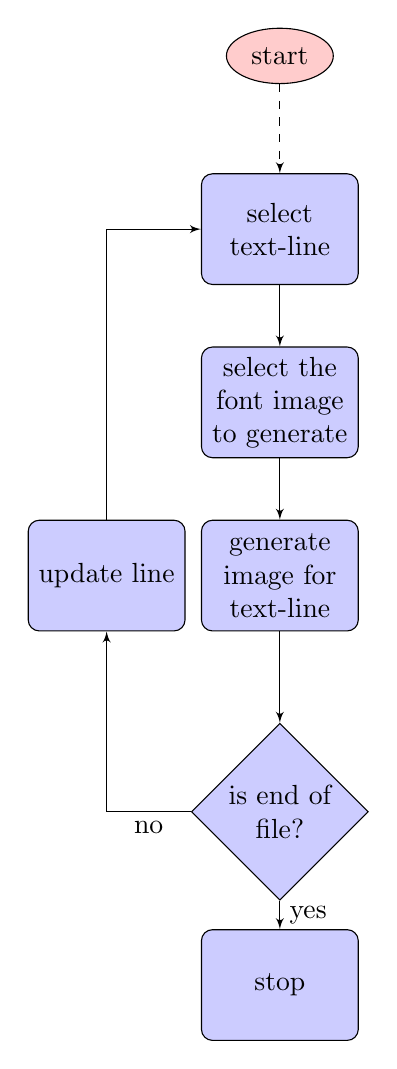
\begin{tikzpicture}[node distance = 2.2cm, auto]

% Place nodes
\node [cloud] (start) {start};
\node [block, below of=start] (init) {select text-line};
%\node [cloud, right of=init] (system) {system};
\node [block, below of=init] (identify) {select the font image to generate};
\node [block, below of=identify] (evaluate) {generate image for text-line};
\node [block, left of=evaluate, node distance=2.2cm] (update) {update line};
\node [decision, below of=evaluate] (decide) {is end of file?};
\node [block, below of=decide, node distance=2.2cm] (stop) {stop};
% Draw edges
\path [line] (init) -- (identify);
\path [line] (identify) -- (evaluate);
\path [line] (evaluate) -- (decide);
\path [line] (decide) -| node [near start] {no} (update);
\path [line] (update) |- (init);
\path [line] (decide) -- node {yes}(stop);
\path [line,dashed] (start) -- (init);
%\path [line,dashed] (system) -- (init);
%\path [line,dashed] (system) |- (evaluate);
\end{tikzpicture}

\caption{The flowchart of generating the \yor image dataset}
\end{figure}

\subsection{Preprocessing stages}
This section discusses the steps involved in the preprocessing stages of the \yor OCR system developed. The performance of these steps is key to the performance of the entire system.

\textbf{Binarization} is the first stage in the \yor OCR methodology. The aim of this stage is to convert the input black and white or color document into a binary representation. We applied Adaptive thresholding as against using Gaussian adaptive because of its performance in situations where it is needed to correct the varying lighting conditions in different areas. The method is used in calculating the magnitude that must be exceeded for a small region of the image thereby resulting in different values for different regions of the same image. 

\textbf{Skew estimation} was applied to attempt to horizontally restore any distorted \yor image dataset. This is done by using Ocropy Python Toolkit to experiment with different angles. The algorithm produces an excellent result because at the point the image is properly aligned, there is a tremendous imbalance between rows with text and the blanks in between them. When the image is rotated, the divergence is blended.

\textbf{Page segmentation:} Page segmentation helps indicate the zones of interest to be recognized on the scanned page. The RAST (Recognition by Adaptive Subdivision of Transformation Space) algorithm was adopted because it is fast and robust compared to the other algorithms. 

\subsection{The \yor OCR LSTM Architecture}
A single LSTM network (also known as Vanilla LSTM) depicted in section 2.1 is adopted for the work. The columns of \yor image data pixels are the inputs to the network. In a sequential manner from left to right, these columns are input into the network. Each possible letters are then scored, with the highest matching the letter. As the columns say letter \textit{\`{A}} are fed into the network, then it is expected that there will be a spike from the \textit{\`{A}} output.

Figure 5 shows the system architecture of the LSTM-based recognizer that was used for the Optical Character Recognition of \yor printed text images. Fully Connected (FC) layers connect every neuron in one layer to every neuron in the succeeding layer. The Rectified Linear Units (ReLUs) - which builds non-linearity in the network - when combined with FC, extracted the important features from the image dataset. The 1D-LSTM-based OCR system which is adapted for the \yor OCR model uses a small number of tunable parameters. One important parameter is the number of LSTM cells in the hidden layer(s) and the number of hidden layers. In this work, only one hidden layer with 200 LSTM memory cells in each of right-to-left and left-to-right layers (corresponding to bidirectional mode). Other parameters are learning rate ($10^{-4}$) and the momentum (set to $0.9$). The \textbf{softmax function} normalizes the outputs of each unit to be between $0$ and $1$, just like a sigmoid function. It also used to divide each output such that the total sum of the outputs is equal to $1$. The output of the softmax function is equivalent to a categorical probability distribution, which tells the probability that any of the \yor character set are true.




\begin{figure}[h]
\centering
\includegraphics[width=0.8\linewidth, height=0.2\textheight]{lstm1}
\caption{The network architecture of the \yor sequence model}
\label{fig:lstm1}
\end{figure}
The network was trained for 23,000 iterations and the intermediate models were saved after every 1,000 iterations. This creates a total of 23 models. The training of the model is done by learning from its mistakes. It transcribes the text in a line, then adjusts the weights in the Neural Net to compensate for the errors. Then it does this again for the next line, and the next, and so on. When it gets to the last line of labeled data, it starts over again. As it loops through the training data over and over again, the model gets better and better. The training errors for these iterations are computed, and then the network with the least error was selected as the best network, which is then used to OCR  the \yor test image dataset.


\subsection{Unigram language modelling}
In an effort to find and improve misspelled \yor words in the model developed for the OCR, a Unigram error correction methodology, also known as dictionary-based error correction was conceived. Using this approach, a lexicon or a lookup dictionary from a \yor Bible corpus was used to spell-check OCR recognized words and correct the words that are misspelled. 

This method employed the use of a spell-checker to corrects single-error misspellings which are the predominant source of erroneous recognition in the \yor OCR recognition system. This system rates the candidates for correction according to their correctness probability and then picks the most likely between the original \yor word and the highest-rated candidate. 

Given a word \textit{w}, and the task of finding the correction \textit{c}, the method \q{correction(w)} tries to choose the most likely spelling correction for \textit{w} out of all possible candidate corrections. The approach uses probabilities to rank the possible candidates that maximize the probability that \textit{c} is the intended correction. The candidate with the highest combined probability is chosen using the arguments of the maximal function. 

\subsection{Implementation Environment}

The model was trained with the open-source OCRopus framework, a free document analysis and optical character recognition library \cite{breuel2008ocropus}. It transcribes the image in a line, then adjusts the weights in the Neural Net to compensate for the errors. Then it does this again for the next line, and the next, and so on. When it gets to the last line of labeled data, it starts over again. As it loops through the training data over and over again, the model gets better and better.

\subsection{Performance Metrics}
The \yor OCR accuracy is measured as \q{Character Error Rate (CER) (\%)}, using the \textit{Levenshtein Edit Distance} algorithm. This algorithm is also commonly known as the Edit Distance. It is the ratio between \textit{insertion}, \textit{deletion} and \textit{substitution} errors and the total number of characters. The formula is as shown in Equation 10. Algorithm 3.1 shows the algorithm used in evaluating the system.

\begin{equation}\label{key}
\text{Character Error Rate (CER)} = \frac{Insertion + Deletion + Substitution}{\text{Total Character}} \times 100 
\end{equation}

\clearpage

Algorithm 3.1: The Algorithm to calculate the Character Error Rate
\begin{algorithm}[H]
\caption{Calculation of Character Error Rate (CER) with Levenshtein Edit Distance
	\label{alg:packed-dna-hamming}}
\begin{algorithmic}[1]
	% \Require{$x$ and $y$ are packed \DNA{} strings of equal length $n$}
	\Statex
	\Function{Edit Distance}{Reference r, Hypothesis h}
	
	%\Let{$z$}{$x \oplus y$} \Comment{$\oplus$: bitwise exclusive-or}
	%\Let{$\delta$}{$0$}
	
	\State $int[|r| +1][|h| + 1] D$  \Comment{Initialisation}
	\For{($i=0; i \leq |r|;i++)$} 
	\For{($j=0; j \leq |h|;j++)$} 
	\If {i==0}
	\State {$D[0][j]$}{$j$}
	\ElsIf{j==0}
	\State {$D[i][0]$}{$i$}                
	\EndIf
	\EndFor
	\EndFor
	\For{($i=1; i \leq |r|;i++)$}   \Comment{Calculation}
	\For{($j=1; j \leq |h|;j++)$} 
	\If {r[i-1] == h[j-1]}
	\Let {$D[i][j]$}{$D[i-1][j-1]$}
	\Else
	\Let {$sub$}{$D[i-1][j-1]+1$}
	\Let {$ins$}{$D[i][j-1]+1$}    
	\Let {$del$}{$D[i-1][j]+1$}    
	\Let {$D[i][j]$}{$min(sub,ins,del)$}    
	\EndIf
	\EndFor
	\EndFor
	
	
	\State \Return{$D[|r|][|h|]$}
	\EndFunction
\end{algorithmic}
\end{algorithm}

The algorithm that is used in computing the Character Error Rate is based on dynamic programming, a technique used in breaking down a complex problem into sub-problem to avoid computing multiple time the same sub-problem. It basically involves using past knowledge to make solving a future problem easier. The main challenge in this approach is whether the cheapest way to convert one string into another involves a final add, remove, or change. Hence, the evaluation of all the three possibilities and the return of the minimum distance from among the three.

In each case, the algorithm recursively computes the distance (number of adds, removes, and changes) required to \q{set up} a final add, a final remove, or a final change. Then, add one to the \q{add distance} and the \q{remove distance} to account for the final add or remove. For the \q{change distance}, one is added only if the final characters in the strings are different (if not, no final change is required).

\subsection{Training the model}
The LSTM networks model developed for optical character recognition of \yor printed images make use of supervised learning where the set of sample pairs containing input \yor text-line images and output ground truth transcription of the image are shown to the network. Through the backpropagation algorithm, the resulting output predictions are then compared with the ground truth. The mean square error is calculated over the entire dataset and the intermediate weights are adjusted using learning rate of $10^{-5}$ until the error decayed sufficiently. At $313$ and $314$ number of iterations, the number of characters in error through the network stands at $226$ and $221$ respectively as shown in Figure 6.

The training of the model is achieved by learning from its past mistakes. It extracts the text in the image, then re-adjusts the weights in the LSTM network to nullify for the errors. Then the iteration continues for the next line, and the next, and so on until it gets to the last line of labeled data and then starts again. As it iterates through the training data, the network gets better. The model shows the character error rate of $1.64\%$ and $1.33\%$ at $103,689$ and $103,690$ number of iterations respectively which is an improvement from the earlier reported iterations.

\begin{figure}[h]
\centering
\includegraphics[width=1.1\linewidth]{train2}
\caption{A screen-shot of the model training.}
\label{fig:train2}
\end{figure}

\section{Results}

\subsection{Convergence error rate as training progresses}
2000 labeled images were used as training data and the other 2000 was held out for test and validation dataset. The models were saved at every 1000th loop and this helps in evaluating the performance of the model as it learns. Figure 7 shows the plot of the number of iteration to the character error rate. The convergence error rate starts at a high value (above 20\%) but quickly reduces to about 7.1\% after 6,700 iterations, then spikes to over 3\% at 7,100. It eventually converges to a minimum of 1.33\% at 16,000 iterations.

The network first learns to recognize spaces, followed by Latin characters,
then special characters and nally \yor letters with diacritics. Although it learns the spaces and Latin characters contained in the image quickly, it
continues to make mistakes again later during training. This happens as it
starts picking up special characters, and \yor letters with diacritics, some
of which are confusable with the lower case Latin letters. The transition from learning spaces and Latin letters to learning \yor letters explains the spike from 2.5\% at 6,700 iterations to 3\% at 7,100 iterations.

\begin{figure}[H]
	\centering
	\includegraphics[width=1.1\linewidth]{trainvalidation}
	\caption{Character Error Rate for Training Dataset and Validation
		Dataset vs number of iterations during training.}
	\label{fig:trainvalidation}
\end{figure}

\subsection{Recognition output}
The recognition output of the \yor OCR system without the spell-check correction engine is shown in Figure 8. The upper section designated as \q{original text} shows the ground-truth of the image file sent to the \yor OCR system while the lower section designated as \q{word recognition} shows the corresponding output from the \yor OCR system. The grayed out part of both section indicates words wherein some or all characters where altered. In the same vein, Figure 9 shows the recognition output of the \yor OCR system with the spell-checking correction engine. The upper section designated as "original text" shows the ground-truth of the image file sent to the \yor OCR system while the lower section designated as \q{language modelling} shows the corresponding output from the \yor OCR system. The grayed out part of both section indicates words wherein some or all characters where altered.

\begin{figure}
\centering
\includegraphics[width=0.7\linewidth]{combineResult1}
\caption{The recognition output of the Yor\`{u}b\'{a} OCR system without the spell-check model.}
\label{fig:combineresult1}
\end{figure}

\begin{figure}
\centering
\includegraphics[width=0.7\linewidth]{combineResult2}
\caption{The recognition output of the Yor\`{u}b\'{a} OCR system with the spelling checker model}
\label{fig:combineresult1}
\end{figure}

\subsection{Performance evaluation results}
There are two test datasets used in the evaluation process. The first dataset consists of 30\% of images generated from the Times New Roman font of the \yor Bible that was not used for training the \yor OCR systems. The total number of text-line images are 740 and the total number of characters is 20462. The second dataset consists 758 text-line images from DejaVuSans font style and 779 text-line images of Ariel font style both generated from the \yor Bible. The results from the model as shown in Table 5, show character error rate of 3.138\% for Times New Roman font, 7.435\% for DejaVuSans font and 15.141\% for Ariel font. The top confusions in applying each of the three font styles are also shown in Table 5. Although modern OCR systems claim above 97 \% character accuracy for popular scripts like Arabic, for example. However, for the same data with low-resolution images or uncommon character set, this claim can drop to lower than 70 \%. It is therefore difficult to directly use the results generated from OCR system for other tasks (such as indexing for textual search and machine translation) without expensive editing.  This Standard \yor OCR model is also not an exception. 

The evaluation of the system after the Spell-checking corrector has been introduced shows a considerable drop in the character error rates. The results as shown in Table 6 shows a character error rate of 3.138\% for Times New Roman font, 7.435\% for DejaVuSans font and 15.141\% for Ariel font. The word \q{\d{S}\`{u}gb\d{\'{o}}n} was recognised as \q{\`{u}gb\d{\'{o}}n} by the \yor OCR model but was corrected with the introduction of the corrector. Another example is the word "g\d{\'{e}}g\d{\'{e}}" which was transcribed as "g\d{e}g\d{e}" but corrected by the spell-checker.

\begin{table}
%\begin{minipage}[c][\textheight]{\textwidth}
\centering
{\caption{The Performance of the Model on Different Fonts}\label{utterance structure} \smallskip}
\begin{tabular}{l p{2.5cm} p{2.0cm} p{2.0cm} r}\toprule[0.01cm]
	Font & Errors  & Total&CER&Top Character \bigstrut \\[2ex] \toprule[0.01cm]
	Times Roman & 642 & 20462 & 3.138\%  & (38, 'i', '\`{\i}')\bigstrut \\[2ex]
	DejaVuSans  & 1560 & 20982 & 7.435\%  & (262, '\'{\i}', 'i' )\bigstrut \\[2ex]
	Ariel       & 3266 & 21570 & 15.141\% & (161, '\'{\i}', 'i')\bigstrut \\[2ex]
	\hline
\end{tabular}
%\end{minipage}
\end{table}

 

\begin{table}
%\begin{minipage}[c][\textheight]{\textwidth}
\centering
{\caption{The Performance of the Model plus Introduction of Spelling checker on Different Fonts}\label{utterance structure} \smallskip}
\begin{tabular}{l p{3.0cm} p{3.0cm} r}\toprule[0.01cm]
	Font & Errors & Total&CER \bigstrut \\[2ex] \toprule[0.01cm]
	Times Roman & 242  & 20462 & 1.182\%  \bigstrut \\[2ex]
	DejaVuSans  & 860 & 20982 & 4.098\% \bigstrut \\[2ex]
	Ariel       & 1266 & 21570 & 5.87\% \bigstrut \\[2ex]
	\hline
\end{tabular}
%\end{minipage}
\end{table}

When compared with the work of \cite{breuel2013high} which use similar architecture - bidirectional LSTM networks - to the problem of machine-printed Latin and Fraktur recogntion, we observed that this model compete favorably.  Though their result achieved a better recognition error rate of 0.6\% on English test-set, the performance will be grossly inadequate if we are to use it for \yor machine-printed images which is a tone language. 

\section{Conclusion and Future Scope of Work}
The performance of the model shows that the farther away an image text font is from the font(s) used in training the network, the higher the character error rate of the recognition. 

There are numerous ways in which the work reported can be further extended. The performance of the \yor OCR system can be improved by developing a more robust language model which can serve as an error correction subsystem towards a drive for a better output. Furthermore, the LSTM-based OCR reported for \yor can be extended further to documents with multiple font styles and sizes and to other languages with similar characterization.
\clearpage



\section*{References}

\bibliography{mybibfile}

\end{document}